\documentclass{standalone}
\usepackage{tikz}
\usetikzlibrary{patterns}
\usetikzlibrary{positioning}
\usetikzlibrary{patterns, positioning}
\usetikzlibrary{shapes.misc}
\usepackage[outline]{contour}
\contourlength{1.5pt} 
\usetikzlibrary{calc}
        \usepackage{relsize}
        \tikzset{fontscale/.style = {font=\relsize{#1}}}

\begin{document}
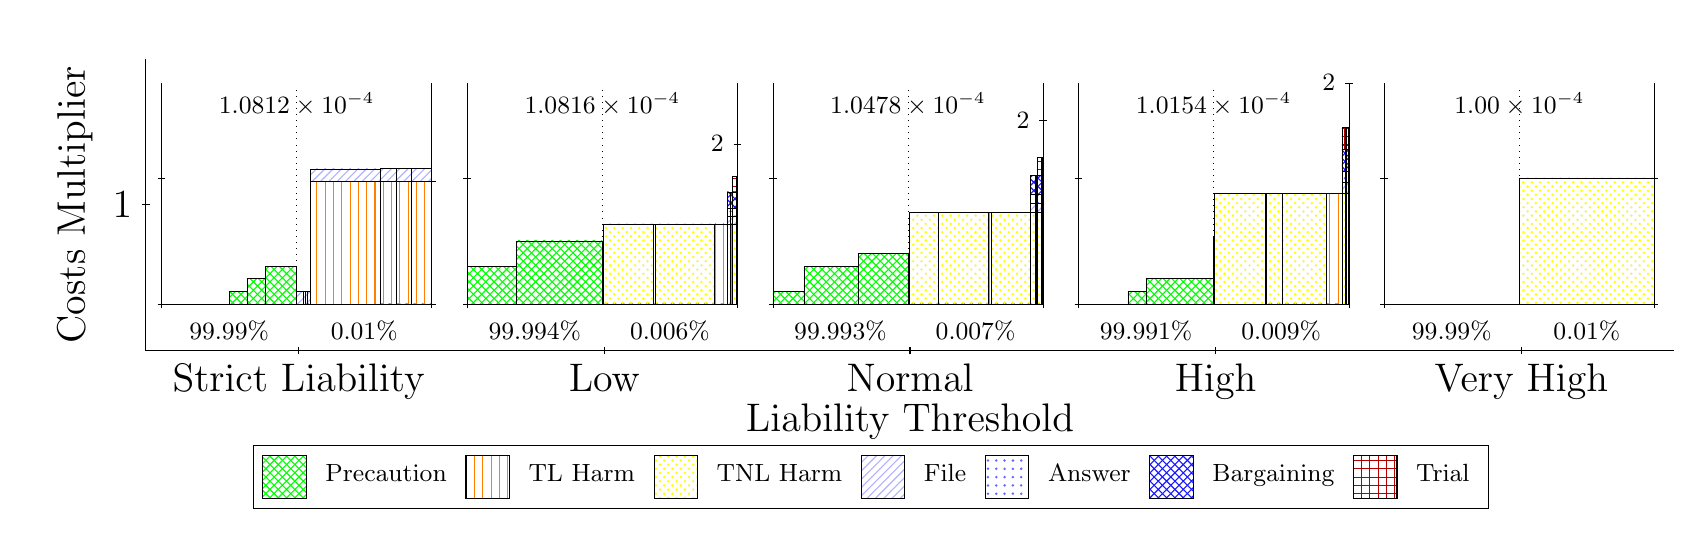
\begin{tikzpicture}
\clip(-0.5,-1.1) rectangle +(20.91,6.2);
\draw[black] (1,1) -- (1,4.7);
\node[rotate=90, fontscale=2, anchor=center] at (0.1, 2.85) {Costs Multiplier};
\draw[black] (0.95,2.85) -- (1.05,2.85);
\node[fontscale=2, anchor=east] at (0.95, 2.85) {1};

\draw[black] (1,1) -- (20.41,1);
\node[fontscale=2, anchor=center] at (10.705, 0.1) {Liability Threshold};
\draw[black] (2.941,0.95) -- (2.941,1.05);
\node[fontscale=2, anchor=north] at (2.941, 0.95) {Strict Liability};
\draw[black] (6.823,0.95) -- (6.823,1.05);
\node[fontscale=2, anchor=north] at (6.823, 0.95) {Low};
\draw[black] (10.705,0.95) -- (10.705,1.05);
\node[fontscale=2, anchor=north] at (10.705, 0.95) {Normal};
\draw[black] (14.587,0.95) -- (14.587,1.05);
\node[fontscale=2, anchor=north] at (14.587, 0.95) {High};
\draw[black] (18.469,0.95) -- (18.469,1.05);
\node[fontscale=2, anchor=north] at (18.469, 0.95) {Very High};


\draw[pattern=crosshatch, pattern color=green,draw=black,very thin] (2.058,1.592) rectangle (2.2894,1.7521);
\draw[pattern=crosshatch, pattern color=green,draw=black,very thin] (2.2894,1.592) rectangle (2.5213,1.9122);
\draw[pattern=crosshatch, pattern color=green,draw=black,very thin] (2.5213,1.592) rectangle (2.916,2.0723);
\draw[pattern=north east lines, pattern color=blue!30,draw=black,very thin] (2.916,1.592) rectangle (3.004,1.748);
\draw[pattern=crosshatch, pattern color=green,draw=black,very thin] (3.004,1.592) rectangle (3.0278,1.592);
\draw[pattern=north east lines, pattern color=blue!30,draw=black,very thin] (3.004,1.592) rectangle (3.0278,1.748);
\draw[pattern=crosshatch, pattern color=green,draw=black,very thin] (3.0278,1.592) rectangle (3.0516,1.592);
\draw[pattern=north east lines, pattern color=blue!30,draw=black,very thin] (3.0278,1.592) rectangle (3.0516,1.748);
\draw[pattern=crosshatch, pattern color=green,draw=black,very thin] (3.0516,1.592) rectangle (3.0921,1.592);
\draw[pattern=north east lines, pattern color=blue!30,draw=black,very thin] (3.0516,1.592) rectangle (3.0921,1.748);
\draw[pattern=vertical lines, pattern color=orange,draw=black,very thin] (3.0921,1.592) rectangle (3.9728,3.1519);
\draw[pattern=north east lines, pattern color=blue!30,draw=black,very thin] (3.0921,3.1519) rectangle (3.9728,3.3079);
\draw[pattern=crosshatch, pattern color=green,draw=black,very thin] (3.9728,1.592) rectangle (4.1845,1.592);
\draw[pattern=vertical lines, pattern color=orange,draw=black,very thin] (3.9728,1.592) rectangle (4.1845,3.152);
\draw[pattern=north east lines, pattern color=blue!30,draw=black,very thin] (3.9728,3.152) rectangle (4.1845,3.308);
\draw[pattern=crosshatch, pattern color=green,draw=black,very thin] (4.1845,1.592) rectangle (4.3686,1.592);
\draw[pattern=vertical lines, pattern color=orange,draw=black,very thin] (4.1845,1.592) rectangle (4.3686,3.152);
\draw[pattern=north east lines, pattern color=blue!30,draw=black,very thin] (4.1845,3.152) rectangle (4.3686,3.308);
\draw[pattern=crosshatch, pattern color=green,draw=black,very thin] (4.3686,1.592) rectangle (4.632,1.592);
\draw[pattern=vertical lines, pattern color=orange,draw=black,very thin] (4.3686,1.592) rectangle (4.632,3.152);
\draw[pattern=north east lines, pattern color=blue!30,draw=black,very thin] (4.3686,3.152) rectangle (4.632,3.308);
\node[font=\small,text=black,anchor=north] at (2.916, 4.4) {$1.0812\times 10^{-4}$};
\draw[black,very thin] (1.2,1.592) -- (1.2,4.4);
\draw[black,very thin] (1.15,1.592) -- (1.25,1.592);
\node[font=\small,text=black, anchor=west] at (1.15, 1.592) {};
\draw[black,very thin] (1.15,3.193) -- (1.25,3.193);
\node[font=\small,text=black, anchor=west] at (1.15, 3.193) {};

\draw[black,dotted,very thin] (2.916,1.6762) -- (2.916,4.3158);
\draw[black,very thin] (4.632,1.592) -- (4.632,4.4);
\draw[black,very thin] (4.582,1.592) -- (4.682,1.592);
\node[font=\small,text=black, anchor=east] at (4.582, 1.592) {\contour{white}{}};
\draw[black,very thin] (4.582,3.1519) -- (4.682,3.1519);
\node[font=\small,text=black, anchor=east] at (4.582, 3.1519) {\contour{white}{}};

\draw[black,very thin] (1.2,1.592) -- (4.632,1.592);
\draw[black,very thin] (1.2,1.542) -- (1.2,1.642);
\node[font=\small,text=black, anchor=north] at (1.2, 1.542) {};
\draw[black,very thin] (4.632,1.542) -- (4.632,1.642);
\node[font=\small,text=black, anchor=north] at (4.632, 1.542) {};

\node[font=\small,text=black,anchor=south] at (2.058, 0.992) {99.99\%};
\node[font=\small,text=black,anchor=south] at (3.774, 0.992) {0.01\%};

\draw[pattern=crosshatch, pattern color=green,draw=black,very thin] (5.082,1.592) rectangle (5.7085,2.0723);
\draw[pattern=crosshatch, pattern color=green,draw=black,very thin] (5.7085,1.592) rectangle (6.798,2.3925);
\draw[pattern=crosshatch, pattern color=green,draw=black,very thin] (6.798,1.592) rectangle (6.8067,1.592);
\draw[pattern=north east lines, pattern color=blue!30,draw=black,very thin] (6.798,1.592) rectangle (6.8067,1.6936);
\draw[pattern=dots,  pattern color=blue!60,draw=black,very thin] (6.798,1.6936) rectangle (6.8067,1.7952);
\draw[pattern=crosshatch,      pattern color=blue!90,draw=black,very thin] (6.798,1.7952) rectangle (6.8067,1.9983);
\draw[pattern=crosshatch, pattern color=green,draw=black,very thin] (6.8067,1.592) rectangle (6.8152,1.592);
\draw[pattern=north east lines, pattern color=blue!30,draw=black,very thin] (6.8067,1.592) rectangle (6.8152,1.6936);
\draw[pattern=dots,  pattern color=blue!60,draw=black,very thin] (6.8067,1.6936) rectangle (6.8152,1.7952);
\draw[pattern=crosshatch,      pattern color=blue!90,draw=black,very thin] (6.8067,1.7952) rectangle (6.8152,1.9983);
\draw[pattern=grid,            pattern color=red!70!black,draw=black,very thin] (6.8067,1.9983) rectangle (6.8152,2.2014);
\draw[pattern=crosshatch, pattern color=green,draw=black,very thin] (6.8152,1.592) rectangle (7.4506,1.592);
\draw[pattern=crosshatch dots, pattern color=yellow,draw=black,very thin] (6.8152,1.592) rectangle (7.4506,2.6077);
\draw[pattern=crosshatch, pattern color=green,draw=black,very thin] (7.4506,1.592) rectangle (7.4681,1.592);
\draw[pattern=vertical lines, pattern color=orange,draw=black,very thin] (7.4506,1.592) rectangle (7.4681,2.6077);
\draw[pattern=crosshatch, pattern color=green,draw=black,very thin] (7.4681,1.592) rectangle (8.2135,1.5921);
\draw[pattern=crosshatch dots, pattern color=yellow,draw=black,very thin] (7.4681,1.5921) rectangle (8.2135,2.6077);
\draw[pattern=crosshatch, pattern color=green,draw=black,very thin] (8.2135,1.592) rectangle (8.3872,1.5921);
\draw[pattern=vertical lines, pattern color=orange,draw=black,very thin] (8.2135,1.5921) rectangle (8.3872,2.6077);
\draw[pattern=crosshatch, pattern color=green,draw=black,very thin] (8.3872,1.592) rectangle (8.4233,1.592);
\draw[pattern=crosshatch dots, pattern color=yellow,draw=black,very thin] (8.3872,1.592) rectangle (8.4233,2.6077);
\draw[pattern=north east lines, pattern color=blue!30,draw=black,very thin] (8.3872,2.6077) rectangle (8.4233,2.7092);
\draw[pattern=dots,  pattern color=blue!60,draw=black,very thin] (8.3872,2.7092) rectangle (8.4233,2.8108);
\draw[pattern=crosshatch,      pattern color=blue!90,draw=black,very thin] (8.3872,2.8108) rectangle (8.4233,3.0139);
\draw[pattern=crosshatch, pattern color=green,draw=black,very thin] (8.4233,1.592) rectangle (8.4506,1.592);
\draw[pattern=vertical lines, pattern color=orange,draw=black,very thin] (8.4233,1.592) rectangle (8.4506,2.6077);
\draw[pattern=north east lines, pattern color=blue!30,draw=black,very thin] (8.4233,2.6077) rectangle (8.4506,2.7092);
\draw[pattern=dots,  pattern color=blue!60,draw=black,very thin] (8.4233,2.7092) rectangle (8.4506,2.8108);
\draw[pattern=crosshatch,      pattern color=blue!90,draw=black,very thin] (8.4233,2.8108) rectangle (8.4506,3.0139);
\draw[pattern=crosshatch, pattern color=green,draw=black,very thin] (8.4506,1.592) rectangle (8.498,1.592);
\draw[pattern=crosshatch dots, pattern color=yellow,draw=black,very thin] (8.4506,1.592) rectangle (8.498,2.6077);
\draw[pattern=north east lines, pattern color=blue!30,draw=black,very thin] (8.4506,2.6077) rectangle (8.498,2.7092);
\draw[pattern=dots,  pattern color=blue!60,draw=black,very thin] (8.4506,2.7092) rectangle (8.498,2.8108);
\draw[pattern=crosshatch,      pattern color=blue!90,draw=black,very thin] (8.4506,2.8108) rectangle (8.498,3.0139);
\draw[pattern=grid,            pattern color=red!70!black,draw=black,very thin] (8.4506,3.0139) rectangle (8.498,3.2171);
\draw[pattern=crosshatch, pattern color=green,draw=black,very thin] (8.498,1.592) rectangle (8.514,1.592);
\draw[pattern=vertical lines, pattern color=orange,draw=black,very thin] (8.498,1.592) rectangle (8.514,2.6077);
\draw[pattern=north east lines, pattern color=blue!30,draw=black,very thin] (8.498,2.6077) rectangle (8.514,2.7092);
\draw[pattern=dots,  pattern color=blue!60,draw=black,very thin] (8.498,2.7092) rectangle (8.514,2.8108);
\draw[pattern=crosshatch,      pattern color=blue!90,draw=black,very thin] (8.498,2.8108) rectangle (8.514,3.0139);
\draw[pattern=grid,            pattern color=red!70!black,draw=black,very thin] (8.498,3.0139) rectangle (8.514,3.2171);
\node[font=\small,text=black,anchor=north] at (6.798, 4.4) {$1.0816\times 10^{-4}$};
\draw[black,very thin] (5.082,1.592) -- (5.082,4.4);
\draw[black,very thin] (5.032,1.592) -- (5.132,1.592);
\node[font=\small,text=black, anchor=west] at (5.032, 1.592) {};
\draw[black,very thin] (5.032,3.193) -- (5.132,3.193);
\node[font=\small,text=black, anchor=west] at (5.032, 3.193) {};

\draw[black,dotted,very thin] (6.798,1.6762) -- (6.798,4.3158);
\draw[black,very thin] (8.514,1.592) -- (8.514,4.4);
\draw[black,very thin] (8.464,3.6233) -- (8.564,3.6233);
\node[font=\small,text=black, anchor=east] at (8.464, 3.6233) {\contour{white}{2}};

\draw[black,very thin] (5.082,1.592) -- (8.514,1.592);
\draw[black,very thin] (5.082,1.542) -- (5.082,1.642);
\node[font=\small,text=black, anchor=north] at (5.082, 1.542) {};
\draw[black,very thin] (8.514,1.542) -- (8.514,1.642);
\node[font=\small,text=black, anchor=north] at (8.514, 1.542) {};

\node[font=\small,text=black,anchor=south] at (5.94, 0.992) {99.994\%};
\node[font=\small,text=black,anchor=south] at (7.656, 0.992) {0.006\%};

\draw[pattern=crosshatch, pattern color=green,draw=black,very thin] (8.964,1.592) rectangle (9.3587,1.7521);
\draw[pattern=crosshatch, pattern color=green,draw=black,very thin] (9.3587,1.592) rectangle (10.053,2.0723);
\draw[pattern=crosshatch, pattern color=green,draw=black,very thin] (10.053,1.592) rectangle (10.68,2.2324);
\draw[pattern=crosshatch, pattern color=green,draw=black,very thin] (10.68,1.592) rectangle (10.688,1.592);
\draw[pattern=north east lines, pattern color=blue!30,draw=black,very thin] (10.68,1.592) rectangle (10.688,1.7085);
\draw[pattern=dots,  pattern color=blue!60,draw=black,very thin] (10.68,1.7085) rectangle (10.688,1.8251);
\draw[pattern=crosshatch,      pattern color=blue!90,draw=black,very thin] (10.68,1.8251) rectangle (10.688,2.0582);
\draw[pattern=crosshatch, pattern color=green,draw=black,very thin] (10.688,1.592) rectangle (10.691,1.592);
\draw[pattern=north east lines, pattern color=blue!30,draw=black,very thin] (10.688,1.592) rectangle (10.691,1.7086);
\draw[pattern=dots,  pattern color=blue!60,draw=black,very thin] (10.688,1.7086) rectangle (10.691,1.8251);
\draw[pattern=crosshatch,      pattern color=blue!90,draw=black,very thin] (10.688,1.8251) rectangle (10.691,2.0582);
\draw[pattern=crosshatch, pattern color=green,draw=black,very thin] (10.691,1.592) rectangle (10.697,1.592);
\draw[pattern=north east lines, pattern color=blue!30,draw=black,very thin] (10.691,1.592) rectangle (10.697,1.7085);
\draw[pattern=dots,  pattern color=blue!60,draw=black,very thin] (10.691,1.7085) rectangle (10.697,1.8251);
\draw[pattern=crosshatch,      pattern color=blue!90,draw=black,very thin] (10.691,1.8251) rectangle (10.697,2.0582);
\draw[pattern=grid,            pattern color=red!70!black,draw=black,very thin] (10.691,2.0582) rectangle (10.697,2.2912);
\draw[pattern=crosshatch, pattern color=green,draw=black,very thin] (10.697,1.592) rectangle (10.699,1.592);
\draw[pattern=north east lines, pattern color=blue!30,draw=black,very thin] (10.697,1.592) rectangle (10.699,1.7086);
\draw[pattern=dots,  pattern color=blue!60,draw=black,very thin] (10.697,1.7086) rectangle (10.699,1.8251);
\draw[pattern=crosshatch,      pattern color=blue!90,draw=black,very thin] (10.697,1.8251) rectangle (10.699,2.0582);
\draw[pattern=grid,            pattern color=red!70!black,draw=black,very thin] (10.697,2.0582) rectangle (10.699,2.2913);
\draw[pattern=crosshatch, pattern color=green,draw=black,very thin] (10.699,1.592) rectangle (11.068,1.592);
\draw[pattern=crosshatch dots, pattern color=yellow,draw=black,very thin] (10.699,1.592) rectangle (11.068,2.7574);
\draw[pattern=crosshatch, pattern color=green,draw=black,very thin] (11.068,1.592) rectangle (11.07,1.592);
\draw[pattern=vertical lines, pattern color=orange,draw=black,very thin] (11.068,1.592) rectangle (11.07,2.7574);
\draw[pattern=crosshatch, pattern color=green,draw=black,very thin] (11.07,1.592) rectangle (11.696,1.592);
\draw[pattern=crosshatch dots, pattern color=yellow,draw=black,very thin] (11.07,1.592) rectangle (11.696,2.7574);
\draw[pattern=crosshatch, pattern color=green,draw=black,very thin] (11.696,1.592) rectangle (11.741,1.592);
\draw[pattern=vertical lines, pattern color=orange,draw=black,very thin] (11.696,1.592) rectangle (11.741,2.7574);
\draw[pattern=crosshatch, pattern color=green,draw=black,very thin] (11.741,1.592) rectangle (12.232,1.592);
\draw[pattern=crosshatch dots, pattern color=yellow,draw=black,very thin] (11.741,1.592) rectangle (12.232,2.7574);
\draw[pattern=crosshatch, pattern color=green,draw=black,very thin] (12.232,1.592) rectangle (12.298,1.592);
\draw[pattern=crosshatch dots, pattern color=yellow,draw=black,very thin] (12.232,1.592) rectangle (12.298,2.7574);
\draw[pattern=north east lines, pattern color=blue!30,draw=black,very thin] (12.232,2.7574) rectangle (12.298,2.8739);
\draw[pattern=dots,  pattern color=blue!60,draw=black,very thin] (12.232,2.8739) rectangle (12.298,2.9904);
\draw[pattern=crosshatch,      pattern color=blue!90,draw=black,very thin] (12.232,2.9904) rectangle (12.298,3.2235);
\draw[pattern=crosshatch, pattern color=green,draw=black,very thin] (12.298,1.592) rectangle (12.308,1.592);
\draw[pattern=vertical lines, pattern color=orange,draw=black,very thin] (12.298,1.592) rectangle (12.308,2.7574);
\draw[pattern=north east lines, pattern color=blue!30,draw=black,very thin] (12.298,2.7574) rectangle (12.308,2.8739);
\draw[pattern=dots,  pattern color=blue!60,draw=black,very thin] (12.298,2.8739) rectangle (12.308,2.9904);
\draw[pattern=crosshatch,      pattern color=blue!90,draw=black,very thin] (12.298,2.9904) rectangle (12.308,3.2235);
\draw[pattern=crosshatch, pattern color=green,draw=black,very thin] (12.308,1.592) rectangle (12.314,1.592);
\draw[pattern=crosshatch dots, pattern color=yellow,draw=black,very thin] (12.308,1.592) rectangle (12.314,2.7574);
\draw[pattern=north east lines, pattern color=blue!30,draw=black,very thin] (12.308,2.7574) rectangle (12.314,2.8739);
\draw[pattern=dots,  pattern color=blue!60,draw=black,very thin] (12.308,2.8739) rectangle (12.314,2.9905);
\draw[pattern=crosshatch,      pattern color=blue!90,draw=black,very thin] (12.308,2.9905) rectangle (12.314,3.2235);
\draw[pattern=crosshatch, pattern color=green,draw=black,very thin] (12.314,1.592) rectangle (12.327,1.592);
\draw[pattern=vertical lines, pattern color=orange,draw=black,very thin] (12.314,1.592) rectangle (12.327,2.7574);
\draw[pattern=north east lines, pattern color=blue!30,draw=black,very thin] (12.314,2.7574) rectangle (12.327,2.8739);
\draw[pattern=dots,  pattern color=blue!60,draw=black,very thin] (12.314,2.8739) rectangle (12.327,2.9905);
\draw[pattern=crosshatch,      pattern color=blue!90,draw=black,very thin] (12.314,2.9905) rectangle (12.327,3.2235);
\draw[pattern=crosshatch, pattern color=green,draw=black,very thin] (12.327,1.592) rectangle (12.376,1.592);
\draw[pattern=crosshatch dots, pattern color=yellow,draw=black,very thin] (12.327,1.592) rectangle (12.376,2.7574);
\draw[pattern=north east lines, pattern color=blue!30,draw=black,very thin] (12.327,2.7574) rectangle (12.376,2.8739);
\draw[pattern=dots,  pattern color=blue!60,draw=black,very thin] (12.327,2.8739) rectangle (12.376,2.9904);
\draw[pattern=crosshatch,      pattern color=blue!90,draw=black,very thin] (12.327,2.9904) rectangle (12.376,3.2235);
\draw[pattern=grid,            pattern color=red!70!black,draw=black,very thin] (12.327,3.2235) rectangle (12.376,3.4566);
\draw[pattern=crosshatch, pattern color=green,draw=black,very thin] (12.376,1.592) rectangle (12.382,1.592);
\draw[pattern=vertical lines, pattern color=orange,draw=black,very thin] (12.376,1.592) rectangle (12.382,2.7574);
\draw[pattern=north east lines, pattern color=blue!30,draw=black,very thin] (12.376,2.7574) rectangle (12.382,2.8739);
\draw[pattern=dots,  pattern color=blue!60,draw=black,very thin] (12.376,2.8739) rectangle (12.382,2.9904);
\draw[pattern=crosshatch,      pattern color=blue!90,draw=black,very thin] (12.376,2.9904) rectangle (12.382,3.2235);
\draw[pattern=grid,            pattern color=red!70!black,draw=black,very thin] (12.376,3.2235) rectangle (12.382,3.4566);
\draw[pattern=crosshatch, pattern color=green,draw=black,very thin] (12.382,1.592) rectangle (12.39,1.592);
\draw[pattern=crosshatch dots, pattern color=yellow,draw=black,very thin] (12.382,1.592) rectangle (12.39,2.7574);
\draw[pattern=north east lines, pattern color=blue!30,draw=black,very thin] (12.382,2.7574) rectangle (12.39,2.8739);
\draw[pattern=dots,  pattern color=blue!60,draw=black,very thin] (12.382,2.8739) rectangle (12.39,2.9905);
\draw[pattern=crosshatch,      pattern color=blue!90,draw=black,very thin] (12.382,2.9905) rectangle (12.39,3.2235);
\draw[pattern=grid,            pattern color=red!70!black,draw=black,very thin] (12.382,3.2235) rectangle (12.39,3.4566);
\draw[pattern=crosshatch, pattern color=green,draw=black,very thin] (12.39,1.592) rectangle (12.396,1.592);
\draw[pattern=vertical lines, pattern color=orange,draw=black,very thin] (12.39,1.592) rectangle (12.396,2.7574);
\draw[pattern=north east lines, pattern color=blue!30,draw=black,very thin] (12.39,2.7574) rectangle (12.396,2.8739);
\draw[pattern=dots,  pattern color=blue!60,draw=black,very thin] (12.39,2.8739) rectangle (12.396,2.9905);
\draw[pattern=crosshatch,      pattern color=blue!90,draw=black,very thin] (12.39,2.9905) rectangle (12.396,3.2235);
\draw[pattern=grid,            pattern color=red!70!black,draw=black,very thin] (12.39,3.2235) rectangle (12.396,3.4566);
\node[font=\small,text=black,anchor=north] at (10.68, 4.4) {$1.0478\times 10^{-4}$};
\draw[black,very thin] (8.964,1.592) -- (8.964,4.4);
\draw[black,very thin] (8.914,1.592) -- (9.014,1.592);
\node[font=\small,text=black, anchor=west] at (8.914, 1.592) {};
\draw[black,very thin] (8.914,3.193) -- (9.014,3.193);
\node[font=\small,text=black, anchor=west] at (8.914, 3.193) {};

\draw[black,dotted,very thin] (10.68,1.6762) -- (10.68,4.3158);
\draw[black,very thin] (12.396,1.592) -- (12.396,4.4);
\draw[black,very thin] (12.346,3.9227) -- (12.446,3.9227);
\node[font=\small,text=black, anchor=east] at (12.346, 3.9227) {\contour{white}{2}};

\draw[black,very thin] (8.964,1.592) -- (12.396,1.592);
\draw[black,very thin] (8.964,1.542) -- (8.964,1.642);
\node[font=\small,text=black, anchor=north] at (8.964, 1.542) {};
\draw[black,very thin] (12.396,1.542) -- (12.396,1.642);
\node[font=\small,text=black, anchor=north] at (12.396, 1.542) {};

\node[font=\small,text=black,anchor=south] at (9.822, 0.992) {99.993\%};
\node[font=\small,text=black,anchor=south] at (11.538, 0.992) {0.007\%};

\draw[pattern=crosshatch, pattern color=green,draw=black,very thin] (13.473,1.592) rectangle (13.704,1.7521);
\draw[pattern=crosshatch, pattern color=green,draw=black,very thin] (13.704,1.592) rectangle (14.562,1.9122);
\draw[pattern=north east lines, pattern color=blue!30,draw=black,very thin] (14.562,1.592) rectangle (14.568,1.7324);
\draw[pattern=dots,  pattern color=blue!60,draw=black,very thin] (14.562,1.7324) rectangle (14.568,1.8728);
\draw[pattern=crosshatch,      pattern color=blue!90,draw=black,very thin] (14.562,1.8728) rectangle (14.568,2.1536);
\draw[pattern=grid,            pattern color=red!70!black,draw=black,very thin] (14.562,2.1536) rectangle (14.568,2.4344);
\draw[pattern=crosshatch, pattern color=green,draw=black,very thin] (14.568,1.592) rectangle (14.571,1.592);
\draw[pattern=north east lines, pattern color=blue!30,draw=black,very thin] (14.568,1.592) rectangle (14.571,1.7324);
\draw[pattern=dots,  pattern color=blue!60,draw=black,very thin] (14.568,1.7324) rectangle (14.571,1.8728);
\draw[pattern=crosshatch,      pattern color=blue!90,draw=black,very thin] (14.568,1.8728) rectangle (14.571,2.1536);
\draw[pattern=grid,            pattern color=red!70!black,draw=black,very thin] (14.568,2.1536) rectangle (14.571,2.4344);
\draw[pattern=crosshatch dots, pattern color=yellow,draw=black,very thin] (14.571,1.592) rectangle (15.221,2.996);
\draw[pattern=vertical lines, pattern color=orange,draw=black,very thin] (15.221,1.592) rectangle (15.227,2.996);
\draw[pattern=crosshatch, pattern color=green,draw=black,very thin] (15.227,1.592) rectangle (15.43,1.592);
\draw[pattern=crosshatch dots, pattern color=yellow,draw=black,very thin] (15.227,1.592) rectangle (15.43,2.996);
\draw[pattern=crosshatch, pattern color=green,draw=black,very thin] (15.43,1.592) rectangle (15.436,1.592);
\draw[pattern=vertical lines, pattern color=orange,draw=black,very thin] (15.43,1.592) rectangle (15.436,2.996);
\draw[pattern=crosshatch, pattern color=green,draw=black,very thin] (15.436,1.592) rectangle (15.993,1.592);
\draw[pattern=crosshatch dots, pattern color=yellow,draw=black,very thin] (15.436,1.592) rectangle (15.993,2.996);
\draw[pattern=crosshatch, pattern color=green,draw=black,very thin] (15.993,1.592) rectangle (16.19,1.592);
\draw[pattern=vertical lines, pattern color=orange,draw=black,very thin] (15.993,1.592) rectangle (16.19,2.996);
\draw[pattern=crosshatch dots, pattern color=yellow,draw=black,very thin] (16.19,1.592) rectangle (16.235,2.996);
\draw[pattern=north east lines, pattern color=blue!30,draw=black,very thin] (16.19,2.996) rectangle (16.235,3.1364);
\draw[pattern=dots,  pattern color=blue!60,draw=black,very thin] (16.19,3.1364) rectangle (16.235,3.2768);
\draw[pattern=crosshatch,      pattern color=blue!90,draw=black,very thin] (16.19,3.2768) rectangle (16.235,3.5576);
\draw[pattern=grid,            pattern color=red!70!black,draw=black,very thin] (16.19,3.5576) rectangle (16.235,3.8384);
\draw[pattern=vertical lines, pattern color=orange,draw=black,very thin] (16.235,1.592) rectangle (16.249,2.996);
\draw[pattern=north east lines, pattern color=blue!30,draw=black,very thin] (16.235,2.996) rectangle (16.249,3.1364);
\draw[pattern=dots,  pattern color=blue!60,draw=black,very thin] (16.235,3.1364) rectangle (16.249,3.2768);
\draw[pattern=crosshatch,      pattern color=blue!90,draw=black,very thin] (16.235,3.2768) rectangle (16.249,3.5576);
\draw[pattern=grid,            pattern color=red!70!black,draw=black,very thin] (16.235,3.5576) rectangle (16.249,3.8384);
\draw[pattern=crosshatch, pattern color=green,draw=black,very thin] (16.249,1.592) rectangle (16.268,1.592);
\draw[pattern=crosshatch dots, pattern color=yellow,draw=black,very thin] (16.249,1.592) rectangle (16.268,2.996);
\draw[pattern=north east lines, pattern color=blue!30,draw=black,very thin] (16.249,2.996) rectangle (16.268,3.1364);
\draw[pattern=dots,  pattern color=blue!60,draw=black,very thin] (16.249,3.1364) rectangle (16.268,3.2768);
\draw[pattern=crosshatch,      pattern color=blue!90,draw=black,very thin] (16.249,3.2768) rectangle (16.268,3.5576);
\draw[pattern=grid,            pattern color=red!70!black,draw=black,very thin] (16.249,3.5576) rectangle (16.268,3.8384);
\draw[pattern=crosshatch, pattern color=green,draw=black,very thin] (16.268,1.592) rectangle (16.278,1.592);
\draw[pattern=vertical lines, pattern color=orange,draw=black,very thin] (16.268,1.592) rectangle (16.278,2.996);
\draw[pattern=north east lines, pattern color=blue!30,draw=black,very thin] (16.268,2.996) rectangle (16.278,3.1364);
\draw[pattern=dots,  pattern color=blue!60,draw=black,very thin] (16.268,3.1364) rectangle (16.278,3.2768);
\draw[pattern=crosshatch,      pattern color=blue!90,draw=black,very thin] (16.268,3.2768) rectangle (16.278,3.5576);
\draw[pattern=grid,            pattern color=red!70!black,draw=black,very thin] (16.268,3.5576) rectangle (16.278,3.8384);
\node[font=\small,text=black,anchor=north] at (14.562, 4.4) {$1.0154\times 10^{-4}$};
\draw[black,very thin] (12.846,1.592) -- (12.846,4.4);
\draw[black,very thin] (12.796,1.592) -- (12.896,1.592);
\node[font=\small,text=black, anchor=west] at (12.796, 1.592) {};
\draw[black,very thin] (12.796,3.193) -- (12.896,3.193);
\node[font=\small,text=black, anchor=west] at (12.796, 3.193) {};

\draw[black,dotted,very thin] (14.562,1.6762) -- (14.562,4.3158);
\draw[black,very thin] (16.278,1.592) -- (16.278,4.4);
\draw[black,very thin] (16.228,4.4) -- (16.328,4.4);
\node[font=\small,text=black, anchor=east] at (16.228, 4.4) {\contour{white}{2}};

\draw[black,very thin] (12.846,1.592) -- (16.278,1.592);
\draw[black,very thin] (12.846,1.542) -- (12.846,1.642);
\node[font=\small,text=black, anchor=north] at (12.846, 1.542) {};
\draw[black,very thin] (16.278,1.542) -- (16.278,1.642);
\node[font=\small,text=black, anchor=north] at (16.278, 1.542) {};

\node[font=\small,text=black,anchor=south] at (13.704, 0.992) {99.991\%};
\node[font=\small,text=black,anchor=south] at (15.42, 0.992) {0.009\%};

\draw[pattern=crosshatch dots, pattern color=yellow,draw=black,very thin] (18.444,1.592) rectangle (20.16,3.1931);
\node[font=\small,text=black,anchor=north] at (18.444, 4.4) {$1.00\times 10^{-4}$};
\draw[black,very thin] (16.728,1.592) -- (16.728,4.4);
\draw[black,very thin] (16.678,1.592) -- (16.778,1.592);
\node[font=\small,text=black, anchor=west] at (16.678, 1.592) {};
\draw[black,very thin] (16.678,3.193) -- (16.778,3.193);
\node[font=\small,text=black, anchor=west] at (16.678, 3.193) {};

\draw[black,dotted,very thin] (18.444,1.6762) -- (18.444,4.3158);
\draw[black,very thin] (20.16,1.592) -- (20.16,4.4);
\draw[black,very thin] (20.11,1.592) -- (20.21,1.592);
\node[font=\small,text=black, anchor=east] at (20.11, 1.592) {\contour{white}{}};
\draw[black,very thin] (20.11,3.1931) -- (20.21,3.1931);
\node[font=\small,text=black, anchor=east] at (20.11, 3.1931) {\contour{white}{}};

\draw[black,very thin] (16.728,1.592) -- (20.16,1.592);
\draw[black,very thin] (16.728,1.542) -- (16.728,1.642);
\node[font=\small,text=black, anchor=north] at (16.728, 1.542) {};
\draw[black,very thin] (20.16,1.542) -- (20.16,1.642);
\node[font=\small,text=black, anchor=north] at (20.16, 1.542) {};

\node[font=\small,text=black,anchor=south] at (17.586, 0.992) {99.99\%};
\node[font=\small,text=black,anchor=south] at (19.302, 0.992) {0.01\%};

\coordinate (LegendAnchor) at (10.205000000000002,0);
\begin{scope}[align=center]
\matrix[scale=0.6,draw=black,below=0.2cm of LegendAnchor,nodes={draw},column sep=0.12cm]{
\node[rectangle,draw,minimum width=0.55cm,minimum height=0.55cm,pattern=crosshatch, pattern color=green]{}; &
        \node[draw=none,font=\small]{Precaution}; &
\node[rectangle,draw,minimum width=0.55cm,minimum height=0.55cm,pattern=vertical lines, pattern color=orange]{}; &
        \node[draw=none,font=\small]{TL Harm}; &
\node[rectangle,draw,minimum width=0.55cm,minimum height=0.55cm,pattern=crosshatch dots, pattern color=yellow]{}; &
        \node[draw=none,font=\small]{TNL Harm}; &
\node[rectangle,draw,minimum width=0.55cm,minimum height=0.55cm,pattern=north east lines, pattern color=blue!30]{}; &
        \node[draw=none,font=\small]{File}; &
\node[rectangle,draw,minimum width=0.55cm,minimum height=0.55cm,pattern=dots, pattern color=blue!60]{}; &
        \node[draw=none,font=\small]{Answer}; &
\node[rectangle,draw,minimum width=0.55cm,minimum height=0.55cm,pattern=crosshatch, pattern color=blue!90]{}; &
        \node[draw=none,font=\small]{Bargaining}; &
\node[rectangle,draw,minimum width=0.55cm,minimum height=0.55cm,pattern=grid, pattern color=red!70!black]{}; &
        \node[draw=none,font=\small]{Trial}; \\
};\end{scope}

\end{tikzpicture}
\end{document}